% =============================================================================
\bloco{2}{Money, inflation and fiscal policy}{Kurlat chs.~10--11; Romer ch.~11 \,\textbullet\, 25 points}

\questao{(10 points) Objective items.}

\textbf{a)} (3 points) \emph{Money demand $\times$ welfare.} Baumol--Tobin: a household holds its income $Y>0$ in a bond paying the
nominal rate $i>0$, spends it evenly over the period and withdraws cash in $N$ equal trips at a cost $F>0$ each ($N$ continuous).
The welfare cost of $i>0$, measured as the Bailey area $\int_0^i m(x)\,dx-i\,m(i)$ under the money demand $m(i)$ this problem
generates, is:
\begin{alternativas}
\item $\sqrt{FYi/4}$
\item $\sqrt{2FYi}$
\item $\sqrt{FYi/8}$
\item $\sqrt{FYi/2}$
\end{alternativas}
\gabarito{D}
\begin{sol}
\passo{money demand}{Cash falls linearly from $Y/N$ to $0$ between trips, so $m=Y/(2N)$ and the household minimizes $FN+iY/(2N)$;
the first-order condition $F=iY/(2N^2)$ (second derivative $iY/N^3>0$) gives $N^*=\sqrt{iY/(2F)}$ and $m(i)=\sqrt{FY/(2i)}$.}
\passo{Bailey area}{The integral converges since $m\propto x^{-1/2}$: $W=\int_0^i\sqrt{FY/(2x)}\,dx-i\,m(i)=\sqrt{2FYi}-\sqrt{FYi/2}
=\sqrt{FYi/2}=FN^*$. The first term is the minimized cost $C(i)=FN^*+i\,m(i)$ (envelope theorem: $C'=m$, $C(0^+)=0$); the interest
$i\,m$ is a transfer to the issuer of money, so the loss is the cost of trips, Kurlat's shoe-leather cost $NF$.}
\passo{distractors}{B also counts the forgone interest, a transfer equal to $FN^*$ at the optimum: it is $C(i)=2W$. C takes
the triangle $\tfrac12\,i\,m(i)$. A makes C's mistake and also uses average balances $Y/N$, so $m=\sqrt{FY/i}$ and $\tfrac12\,i\,m=\tfrac12\sqrt{FYi}$.}
\refbib{Kurlat (2020), ch.~10, \S10.4, eqs.~(10.4.1)--(10.4.4); ch.~11, \S11.4, eq.~(11.4.1).}
\end{sol}

\medskip
\textbf{b)} (3 points) \emph{Money $\times$ expectations.} Cagan with perfect foresight and no bubbles, in logs:
$m_t-p_t=-a(p_{t+1}-p_t)$, $a>0$. Money has been constant; at $t=0$ the central bank credibly announces a permanent rise of
$\theta>0$ in the log money supply from date $k\ge1$ on. On impact $p_0$ rises by:
\begin{alternativas}
\item $\big[1-\big(\frac{a}{1+a}\big)^{k}\big]\,\theta$
\item $\frac{1}{1+a}\big(\frac{a}{1+a}\big)^{k}\,\theta$
\item $\big(\frac{a}{1+a}\big)^{k}\,\theta$
\item $\frac{1}{1+a}\big[1-\big(\frac{a}{1+a}\big)^{k}\big]\,\theta$
\end{alternativas}
\gabarito{C}
\begin{sol}
\passo{forward solution}{Solving for $p_t$, $p_t=\frac1{1+a}m_t+\lambda p_{t+1}$, $\lambda\equiv\frac a{1+a}\in(0,1)$; iterating with no
bubbles ($\lambda^np_{t+n}\to0$), $p_t=\frac1{1+a}\sum_{j\ge0}\lambda^jm_{t+j}$, with weights summing to $\frac1{(1+a)(1-\lambda)}=1$.}
\passo{news}{Only $m_j$, $j\ge k$, rise by $\theta$: $\Delta p_0=\frac{\theta}{1+a}\sum_{j\ge k}\lambda^j=\frac{\theta}{1+a}\,
\frac{\lambda^k}{1-\lambda}=\lambda^k\theta$, and $p_t$ rises by $\lambda^{k-t}\theta$ for $t\le k$: prices climb before the money arrives.}
\passo{distractors}{A is the rise still to come, $(1-\lambda^k)\theta$; B treats the rise as temporary, moving only $m_k$; D makes
both mistakes: the rise still to come under a temporary rise, from impact to its peak $\theta/(1+a)$ at date $k$.}
\refbib{Romer (2012), ch.~11, Problem~11.1; Kurlat (2020), ch.~11, Exercise~11.6.}
\end{sol}

\medskip
\textbf{c)} (2 points, T or F) With money demand as in b) and money growth long at $\mu_1$, a credible announcement at $t=0$ that
money growth will fall permanently to $\mu_2<\mu_1$ after date $T\ge1$ leaves inflation at $\mu_1$ until money growth falls.
\gabarito{F}
\begin{sol}
\passo{forward-looking prices}{By b), $p_t-m_t=\frac1{1+a}\sum_{j\ge0}\lambda^j(m_{t+j}-m_t)$, equal to $a\mu_1$ on the old path; the
announcement lowers $m_{t+j}-m_t$ by $(\mu_1-\mu_2)\max\{0,t+j-T\}$, so, by the sums of Question~4(d),
$p_t=m_t+a\mu_1-a(\mu_1-\mu_2)\lambda^{T-t}$ for $0\le t\le T$. Inflation is $\mu_1-a(\mu_1-\mu_2)\lambda^T$ in the announcement period
and $\mu_1-(\mu_1-\mu_2)\lambda^{T-s+1}$ at $1\le s\le T$, always below $\mu_1$: it falls at once.}
\refbib{Romer (2012), ch.~11, Problem~11.1(d); Kurlat (2020), ch.~11, Exercise~11.4.}
\end{sol}

\medskip
\textbf{d)} (2 points, T or F) \emph{Money $\times$ taxes.} With nominal interest income taxed at $\tau\in(0,1)$ and a constant
after-tax real return, the nominal rate rises by more than one point per point of expected inflation, and the before-tax real
rate $i-\pi^e$ rises with $\pi^e$.
\gabarito{T}
\begin{sol}
\passo{Darby effect}{$(1-\tau)i-\pi^e=\bar r$ gives $i=(\bar r+\pi^e)/(1-\tau)$, so $di/d\pi^e=1/(1-\tau)>1$, and $i-\pi^e=(\bar r+\tau\pi^e)/(1-\tau)$
has slope $\tau/(1-\tau)>0$: the tax also falls on the inflation premium. $\tau=0$ restores the one-for-one Fisher effect.}
\refbib{Kurlat (2020), ch.~11, \S11.1, eq.~(11.1.1); Romer (2012), ch.~11, \S11.3 (inflation and the tax system).}
\end{sol}

% -----------------------------------------------------------------------------
\questao{(15 points) Discursive. \emph{Money $\times$ fiscal policy $\times$ expectations: unpleasant arithmetic.} Real money
demand and debt, as shares of GDP, are $m=\kappa e^{-a\pi}$ ($\kappa,a>0$) and $b_{t+1}=(1+r)b_t+d-S_t$, with $r>0$, primary
deficit $d\ge0$ and $b_0>0$; output does not grow, so seigniorage at constant inflation $\pi\ge0$ is $S=\pi m$. The seigniorage
$S_0$ that would hold debt at $b_0$ is below the largest steady-state seigniorage (part a). As in the Brazilian debates of the
1980s, the central bank tightens and the Treasury does not adjust: for $T\ge1$ periods ($t=0,\dots,T-1$) seigniorage is
$S_1\in(0,S_0)$; from $T$ on, debt is held at $b_T$.}

\textbf{a)} (3 points) Characterize the steady states: the link between debt, deficit and seigniorage; the largest seigniorage;
how many inflation rates raise a given $S$, and which to select and why; and the inflation rate $\pi_0$ if debt is stabilized at
once, with bounds in terms of $S_0$ and $\kappa$.
\resolespaco
\begin{sol}
\passo{budget and Laffer curve}{Constant debt requires $S=d+rb$ (deficit plus interest bill), so $S_0=d+rb_0$. At
constant $\pi$, $S(\pi)=\kappa\pi e^{-a\pi}$, $S'(\pi)=\kappa e^{-a\pi}(1-a\pi)$ and $S''(\pi)=-a\kappa e^{-a\pi}(2-a\pi)$: $S$ rises on
$[0,1/a]$ and falls after, $S(0)=0$, $S\to0$ as $\pi\to\infty$, the unique maximum is $S_{\max}=S(1/a)=\kappa/(ae)$, and $S$ is
strictly concave on $[0,2/a)$.}
\passo{two roots, one selected}{For $0<S<S_{\max}$, continuity and strict monotonicity on each side of $1/a$ give exactly one root
$\pi_L(S)\in(0,1/a)$ and one $\pi_H(S)>1/a$ (intermediate value theorem); they merge at $S_{\max}$ and none exists above it. On
the high branch $\pi_H'=1/S'(\pi_H)<0$, so a smaller financing need would raise inflation; like Romer, we select $\pi_L$.}
\passo{properties of $\pi_L$}{Inverse-function rule: $\pi_L'(S)=e^{a\pi_L}/[\kappa(1-a\pi_L)]>0$ and $\pi_L''=-S''/S'^3>0$: inflation is
increasing and strictly convex in the seigniorage it must raise, and $\pi_L'\to\infty$ as $S\to S_{\max}$. As $e^{-1}<e^{-a\pi}<1$ on
$(0,1/a)$, $S/\kappa<\pi_L(S)<eS/\kappa$; so $\pi_0=\pi_L(S_0)$ exists, with $S_0/\kappa<\pi_0<eS_0/\kappa$.}
\intuicao{Inflation taxes real balances; past $\pi=1/a$ the base, shrinking at the semi-elasticity $a$, outweighs the higher rate.}
\refbib{Kurlat (2020), ch.~11, \S11.3, eq.~(11.3.1), and Exercise~11.6; Romer (2012), ch.~11, \S11.9, eqs.~(11.67)--(11.69).}
\rubrica{
\item $S=d+rb$, $S'$, the peak at $1/a$ and $S_{\max}$ derived: 1.5 pts (numerical curve: max.\ half).
\item Two roots proved, low branch justified: 1 pt (roots asserted without monotonicity: 0).
\item $\pi_0$ with its bounds: 0.5 pt.
}
\end{sol}

\textbf{b)} (3 points) Find debt at $T$ and the seigniorage $S_2$ needed from $T$ on in closed form, and describe debt during the
tight phase. Characterize inflation during ($\pi_1$) and after ($\pi_2$) the tight phase; when does $\pi_2$ exist?
\resolespaco
\begin{sol}
\passo{debt}{With $S_t=S_1$ the debt equation has the fixed point $\bar b=(S_1-d)/r$ and $b_{t+1}-\bar b=(1+r)(b_t-\bar b)$, so
$b_T=\bar b+(1+r)^T(b_0-\bar b)=(1+r)^Tb_0+(d-S_1)[(1+r)^T-1]/r$. As $b_0-\bar b=(S_0-S_1)/r>0$, $b_{t+1}-b_t=(1+r)^t(S_0-S_1)>0$:
debt rises ever faster, without bound if the phase never ends.}
\passo{seigniorage and inflation later}{Freezing debt needs $S_2=d+rb_T$ (part a); with $d+r\bar b=S_1$ and $r(b_0-\bar b)=S_0-S_1$,
$S_2=S_1+(1+r)^T(S_0-S_1)$: the tightness gap compounds at $r$. Then $\pi_1=\pi_L(S_1)$ and $\pi_2=\pi_L(S_2)$, which exists iff
$S_2\le S_{\max}$; both obey the bounds of a).}
\intuicao{Seigniorage not collected today is borrowed at $r$, and the interest must be paid with seigniorage forever after.}
\refbib{Kurlat (2020), ch.~11, \S11.3, eq.~(11.3.1).}
\rubrica{
\item $b_T$ by solving the difference equation, and debt rising: 1 pt.
\item $S_2$ in the compounding form: 1 pt (quoted without derivation: max.\ a third).
\item $\pi_1$, $\pi_2$ on the low branch with the existence condition: 1 pt.
}
\end{sol}

\textbf{c)} (3 points) Compare $\pi_2$ with $\pi_0$, and compare the $r$-discounted average inflation
$\bar\pi\equiv\frac{r}{1+r}\sum_{t\ge0}(1+r)^{-t}\pi(t)$ under this policy and under immediate stabilization. Find in closed form the
length $T^*$ of the tight phase beyond which no steady state exists.
\resolespaco
\begin{sol}
\passo{later inflation}{By b), $S_2-S_0=[(1+r)^T-1](S_0-S_1)>0$ for $r>0$, $T\ge1$, $S_1<S_0$; as $\pi_L$ is strictly increasing,
$\pi_1<\pi_0<\pi_2$: lower inflation now is bought with higher inflation forever after.}
\passo{discounted average}{The weights $\frac r{1+r}(1+r)^{-t}$ sum to one, those of $t\ge T$ to $\omega\equiv(1+r)^{-T}$, and
$(1-\omega)S_1+\omega S_2=S_1+\omega(1+r)^T(S_0-S_1)=S_0$: the intertemporal budget fixes discounted seigniorage, and the policy only
re-times it. By strict convexity of $\pi_L$ (Jensen),
\[\bar\pi=(1-\omega)\pi_L(S_1)+\omega\pi_L(S_2)>\pi_L\big((1-\omega)S_1+\omega S_2\big)=\pi_0 .\]}
\passo{collapse}{A steady state exists iff $S_2\le S_{\max}$, i.e.\ $(1+r)^T\le(S_{\max}-S_1)/(S_0-S_1)$:
\[T^*=\frac{\ln[(S_{\max}-S_1)/(S_0-S_1)]}{\ln(1+r)}>0,\qquad S_{\max}=\frac{\kappa}{ae};\]
for $T>T^*$ no inflation rate pays the interest bill.}
\intuicao{The policy only re-times the inflation tax; since each unit of seigniorage costs more inflation than the last, bunching
it later raises average inflation.}
\refbib{Kurlat (2020), ch.~11, \S11.3; Romer (2012), ch.~11, \S11.9; Sargent and Wallace's (1981) unpleasant monetarist arithmetic.}
\rubrica{
\item $S_2>S_0$ and the ordering via the increasing branch: 1 pt (ordering merely asserted: 0 for this line).
\item Unchanged discounted seigniorage and Jensen's inequality: 1 pt.
\item $T^*$ derived, with $T^*>0$: 1 pt.
}
\end{sol}

\textbf{d)} (3 points) Now money demand is forward-looking, $m_t-p_t=-a(p_{t+1}-p_t)$ in logs, with perfect foresight and no
bubbles. Money has long grown at $\mu_1$; at $t=0$ it is credibly announced that $m_t-m_{t-1}=\mu_1$ for $t\le T$ and $\mu_2>\mu_1$
for $t>T$. Find the price level, its jump on announcement and inflation at every date; characterize inflation before $T$ (bounds,
monotonicity, half-life) and the timing of the fall in real balances; read it with $\mu_1=\pi_1$, $\mu_2=\pi_2$.
\resolespaco
\begin{sol}
\passo{forward solution}{By Question~3(b), $p_t-m_t=\frac1{1+a}\sum_{j\ge0}\lambda^j(m_{t+j}-m_t)$, $\lambda\equiv\frac a{1+a}$, and two sums do
the work: $\frac1{1+a}\sum_{j\ge0}j\lambda^j=\frac{\lambda}{(1+a)(1-\lambda)^2}=a$ and $\frac1{1+a}\sum_{j\ge n}(j-n)\lambda^j=a\lambda^n$.}
\passo{price level}{For $t\le T$, $m_{t+j}-m_t=\mu_1j+\Delta\max\{0,t+j-T\}$ with $\Delta\equiv\mu_2-\mu_1>0$; for $t\ge T$ it is $\mu_2j$.
Hence $p_t=m_t+a\mu_1+a\Delta\lambda^{T-t}$ for $0\le t\le T$ and $p_t=m_t+a\mu_2$ for $t\ge T$ (equal at $T$). The old path was
$m_t+a\mu_1$, so $p_0$ jumps up by $a\Delta\lambda^T$.}
\passo{inflation}{With $a(1-\lambda)=\lambda$: $\pi(s)\equiv p_s-p_{s-1}=\mu_1+\Delta\lambda^{T-s+1}$ for $1\le s\le T$ and $\mu_2$ after, so $\mu_1<\pi(s)<\mu_2$,
rising in $s$; the excess $\Delta\lambda^k$, $k$ periods before the switch, halves every $\ln2/\ln(1+1/a)$ periods. Real balances fall by
$a\Delta$ in all, and jump plus excess inflation sum to $a\Delta\lambda^T+\sum_{k=1}^T\Delta\lambda^k=a\Delta$: all of it by $T$. With
$\mu_1=\pi_1$, $\mu_2=\pi_2$ (b--c), inflation exceeds $\pi_1$ throughout the tight phase.}
\intuicao{Expected inflation lowers money demand now, so prices rise before the money does: tight money does not even buy low
inflation meanwhile, and a larger $a$ (higher $\lambda$) pulls inflation further forward.}
\refbib{Romer (2012), ch.~11, Problem~11.1; Kurlat (2020), ch.~11, Exercises~11.4 and 11.6.}
\rubrica{
\item Forward solution and the two sums: 1 pt.
\item Price level, jump and inflation path: 1 pt.
\item Bounds, monotonicity, half-life, fall $a\Delta$ by $T$, read with $\pi_1,\pi_2$: 1 pt (no link to b--c: max.\ half).
}
\end{sol}

\textbf{e)} (3 points) \emph{Parameter analysis.} Sign, with proofs, the effects of $S_1$, $T$, $r$, $d$ (or $b_0$), $\kappa$, $a$ on
$S_2$, $\pi_2$, $\pi_2-\pi_1$, $T^*$ in a table; give the limits $T\to0$, $S_1\to S_0$, $T\to T^*$, $r\to0$, $a\to0$ with their reading;
draw $\pi_2$ against $T$ for two values of $S_1$.
\resolespaco
\begin{sol}
\passo{$S_2$}{From $S_2=S_1+(1+r)^T(S_0-S_1)$, $S_0=d+rb_0$: $\partial_{S_1}S_2=1-(1+r)^T<0$, $\partial_TS_2=(1+r)^T\ln(1+r)(S_0-S_1)>0$,
$\partial_rS_2=T(1+r)^{T-1}(S_0-S_1)+(1+r)^Tb_0>0$, $\partial_dS_2=(1+r)^T>0$, $\partial_{b_0}S_2=r(1+r)^T>0$; $\kappa,a$ do not enter.}
\passo{$\pi_2$ and $\pi_2-\pi_1$}{Implicit differentiation of $\kappa\pi e^{-a\pi}=S$ on the low branch ($1-a\pi>0$):
$\partial_S\pi_L=e^{a\pi}/[\kappa(1-a\pi)]>0$, $\partial_\kappa\pi_L=-G(\pi)/\kappa$, $\partial_a\pi_L=H(\pi)$, with $G\equiv\pi/(1-a\pi)$ and
$H\equiv\pi^2/(1-a\pi)$ positive and increasing on $(0,1/a)$. So $\pi_2$ inherits the signs of $S_2$, falls with $\kappa$, rises with $a$.
Gap: $\partial_{S_1}(\pi_2-\pi_1)=\pi_L'(S_2)[1-(1+r)^T]-\pi_L'(S_1)<0$; $T,r,d,b_0$ move only $\pi_2$; as $\pi_2>\pi_1$, the $\kappa$
effect $-[G(\pi_2)-G(\pi_1)]/\kappa<0$ and the $a$ effect $H(\pi_2)-H(\pi_1)>0$.}
\passo{$T^*$}{$\partial_{S_1}T^*=\big[\frac1{S_0-S_1}-\frac1{S_{\max}-S_1}\big]/\ln(1+r)>0$ as $S_0<S_{\max}$; $d$, $b_0$, $r$ raise $S_0$
and lower the positive numerator, and $r$ raises the denominator: all three lower $T^*$; $\kappa$ raises $S_{\max}$ and $T^*$, $a$
lowers both; $T$ does not enter.}
\passo{limits}{$T\to0$ or $S_1\to S_0$: $S_2\to S_0$, $\pi_2\to\pi_0$ (no tightening, no arithmetic), and $T^*\to\infty$ as $S_1\to S_0$.
$T\to T^*$: $S_2\to S_{\max}$, $\pi_2\to1/a$, $d\pi_2/dT=\pi_L'(S_2)\,\partial_TS_2\to\infty$: a vertical end where the roots merge.
$r\to0$ ($S_1<d$): $S_2\to d$ for all $T$ and $T^*\to\infty$; without compounding, delay is free. $a\to0$: $S_{\max}\to\infty$, and
$\pi_L=(S/\kappa)e^{a\pi_L}$ with $a\pi_L<aeS/\kappa\to0$ gives $\pi_L\to S/\kappa$ (linear Laffer curve, $\bar\pi-\pi_0\to0$); $\lambda\to0$
ends the anticipation of d).}

\par\smallskip\noindent
\begin{minipage}{0.4\linewidth}\centering\small\setlength{\tabcolsep}{4pt}
\begin{tabular}{lcccccc}
\toprule
 & $S_1$ & $T$ & $r$ & $d,b_0$ & $\kappa$ & $a$ \\
\midrule
$S_2$ & $-$ & $+$ & $+$ & $+$ & $0$ & $0$ \\
$\pi_2$ & $-$ & $+$ & $+$ & $+$ & $-$ & $+$ \\
$\pi_2-\pi_1$ & $-$ & $+$ & $+$ & $+$ & $-$ & $+$ \\
$T^*$ & $+$ & $0$ & $-$ & $-$ & $+$ & $-$ \\
\bottomrule
\end{tabular}
\end{minipage}\hfill
\begin{minipage}{0.58\linewidth}\centering
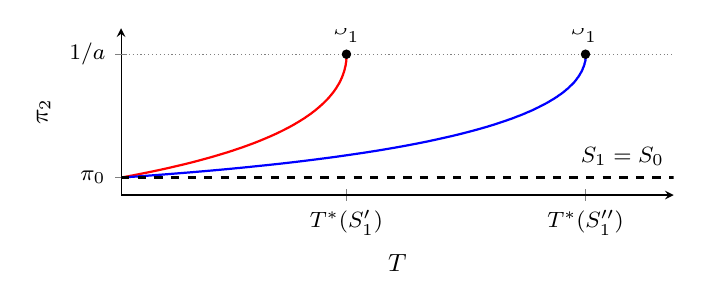
\begin{tikzpicture}
\begin{axis}[width=8.6cm,height=3.7cm,xmin=0,xmax=22,ymin=0.35,ymax=1.12,axis lines=left,xlabel={$T$},ylabel={$\pi_2$},
  xtick={8.972,18.488},xticklabels={$T^*(S_1')$,$T^*(S_1'')$},ytick={0.4308,1},yticklabels={$\pi_0$,$1/a$},
  tick label style={font=\footnotesize},label style={font=\small}]
\addplot[thick,red,domain=0.4308:1,samples=120,variable=\t] ({ln((\t*exp(-\t)-0.12)/0.16)/ln(1.05)},{\t});
\addplot[thick,blue,domain=0.4308:1,samples=120,variable=\t] ({ln((\t*exp(-\t)-0.22)/0.06)/ln(1.05)},{\t});
\addplot[thick,black,dashed,domain=0:22] {0.4308};
\addplot[gray,densely dotted,domain=0:22] {1};
\addplot[only marks,mark=*,mark size=1.5pt] coordinates {(8.972,1) (18.488,1)};
\node[font=\footnotesize,anchor=south] at (axis cs:8.972,1.01) {$S_1'$};
\node[font=\footnotesize,anchor=south] at (axis cs:18.488,1.01) {$S_1''$};
\node[font=\footnotesize,anchor=south east] at (axis cs:22,0.44) {$S_1=S_0$};
\end{axis}
\end{tikzpicture}
\end{minipage}
\passo{graph}{Admissible values, $S_1'<S_1''<S_0$: curves start at $\pi_0$, rise, are convex ($\pi_2''=\pi_L''(\partial_TS_2)^2
+\pi_L'\,\partial_T^2S_2>0$); the tighter one lies above and ends earlier; $S_1=S_0$ is flat.}
\intuicao{Tighter, longer restraint raises later inflation, more so with higher $r$, debt or deficit, and elastic demand hastens
the collapse. With $r$ above growth (here $r>0=g$), restraint without fiscal adjustment postpones inflation and enlarges it.}
\refbib{Kurlat (2020), ch.~11, \S11.3; Romer (2012), ch.~11, \S11.9.}
\rubrica{
\item Signs proved by implicit differentiation: 1 pt (without proofs or reading: max.\ half of the item).
\item Table, limits with proofs, reading: 1 pt.
\item Graph: labelled axes; rising convex curves from $\pi_0$ ordered by $S_1$, vertical at $T^*(S_1)$: 1 pt.
}
\end{sol}
